\documentclass[12pt]{beamer}
\usepackage[utf8]{inputenc}
\usepackage[main=ukrainian,english]{babel}
\usepackage{amsmath}
\usepackage{multicol}
\usetheme{Berkeley}
\logo{
\includegraphics[height=1.5cm]{images/Lviv_Polytechnic} }

\title{Усунення шуму на зображеннях}
\author{Ольга Павлюк}
\subtitle{{ дослідження,  розроблення алгоритмів та програмного забезпечення}}
\institute{Національний університет "Львівська політехніка", кафедра ПЗ}

\date{\today}

\begin{document}

\begin{frame}
	\titlepage
\end{frame}

\begin{frame}
	\frametitle{Зміст} 
	\tableofcontents
\end{frame}

\section{Проблема шуму в зображеннях}
\subsection{Визначення}
\begin{frame}\frametitle{Проблема шуму на зображеннях}
	\begin{block}{Шум}
	випадкові, відсутні на реальному зображенні відхилення інтенсивності
	\end{block}
	\linebreak 
	\pause
	Поширена проблема для цифрових зображень у багатьох галузях.\linebreak
	Виникає при недостатьому освітленні та високій ISO камери. 
	\pause
	\begin{block}{Формальний опис}
		v(i) = u(i) + n(i), де i - піксель зображення \linebreak
		v(i) - спостережене значення, u(i) - справжнє значення \linebreak
		n(i) - значення шуму 
	\end{block}
\end{frame}

\subsection{Характеристики}
\begin{frame}\frametitle{Параметри оцінки алгоритмів}
	\begin{enumerate}
		\item автоматичні: Peak Signal-to-Noise Ratio \linebreak
		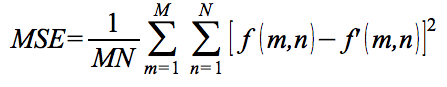
\includegraphics[scale=0.4]{images/mse} \linebreak
		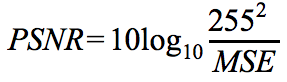
\includegraphics[scale=0.4]{images/psnr} \linebreak
		\item візуальна оцінка: вирішальний критерій вибору алгоритму
	\end{enumerate}
\end{frame}

\subsection{Існуючі алгоритми усунення шуму}
\begin{frame}\frametitle{Існуючі методи усунення шуму}	
	\begin{multicols}{2}
		[
		\begin{center} different image domains \end{center}
		]
		
		алгоритми з патчами\linebreak O(n^{2}) \linebreak
		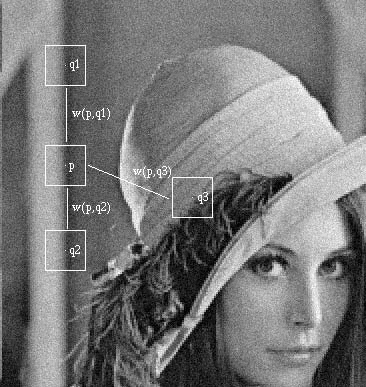
\includegraphics[scale=0.35]{images/patch}
		
		\columnbreak
		
		алгоритми з вейвлетами\linebreak O(n*\log{n}) \linebreak
		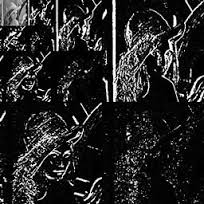
\includegraphics[scale=0.65]{images/dwt}
	\end{multicols}
	
\end{frame}

\begin{frame}\frametitle{Існуючі методи усунення шуму}	
	\begin{multicols}{2}
		[
		\begin{center} different image domains \end{center}
		]
		
		алгоритми з патчами 
		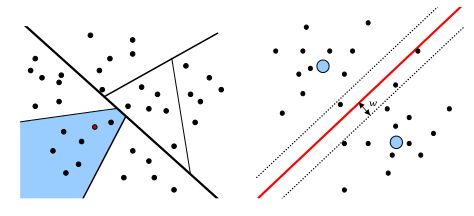
\includegraphics[scale=0.25]{images/cluster} \linebreak
		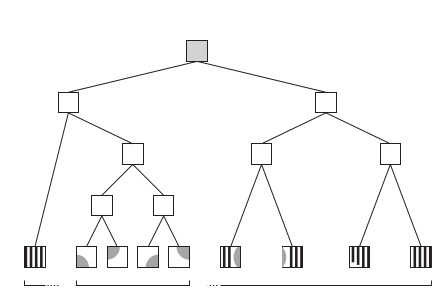
\includegraphics[scale=0.2]{images/patch2} \linebreak
		дерево кластерів: нижча складність, нижча якість
		\columnbreak
		
		алгоритми з вейвлетами
		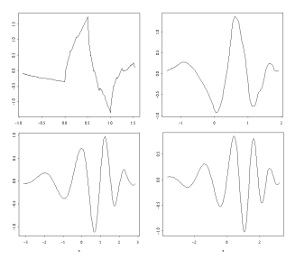
\includegraphics[scale=0.4]{images/waves} \linebreak
		базові функції вейвлета: різна роздільна здатність
	\end{multicols}
\end{frame}

\begin{frame}\frametitle{Вейвлет-алгоритми}
	\begin{enumerate}
		\item виконується рекурсивна декомпозиція сигналу до заданого рівня\linebreak
		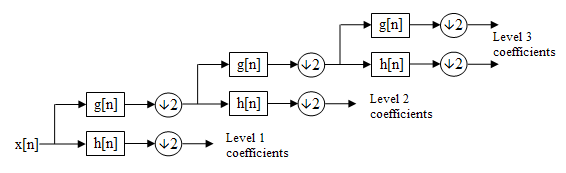
\includegraphics[scale=0.3]{images/filter_bank} \linebreak
		\item коефіцієнти аналізуються "знизу вверх" 
		\item застосовується порогове відсікання (thresholding): \linebreak
		\[
		w(x)= 
		\begin{cases}
		w(x),& \text{if } \mid{w(x)}\mid \geq threshold\\
		0,              & \text{otherwise}
		\end{cases}
		\]
		\item до отриманих коефіцієнтів застосовується зворотнє перетворення
	\end{enumerate}
\end{frame}

\section{Завдання магістерського дослідження}
\begin{frame}\frametitle{Завдання магістерського дослідження}
	\begin{block}{Об'єкт}
		шум на зображеннях
	\end{block}
	\begin{block}{Предмет}
		розробка алгоритму для усунення шуму, що працює в частотній області
	\end{block}
	\begin{block}{Мета}
		розробити алгоритм з лінійно-логарифмічною складністю, який покращує існуючі методи усунення шуму (час роботи + візуальна оцінка)
	\end{block}
\end{frame}


\section{Алгоритм Curvelet Transform}
\begin{frame}\frametitle{Алгоритм Curvelet Transform }
	\begin{enumerate}
		\item один з видів вейвлет-перетворення
		\item усуває шум вздовж кривих
		\item працює у частотній області
		\item складається з кількох незалежних перетворень
	\end{enumerate} 
\end{frame}

\begin{frame}\frametitle{Перетворення Фур'є (Fourier Transform)  }
базовий метод для всіх алгоритмів, що працюють з частотами \linebreak \linebreak  
сигнал можна представити у вигляді суми синусоїд з різними амплітудами та зсувом
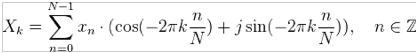
\includegraphics[scale=0.5]{images/fourier_1d} 
\end{frame}

\begin{frame}\frametitle{Перетворення Фур'є (Fourier Transform)  }
	\begin{multicols}{2}
		[ операція згортки (convolution) сигналу з фільтром довільної довжини виконується за лінійний час
		]
		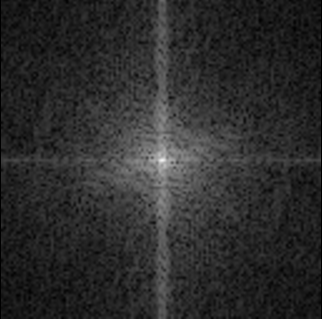
\includegraphics[scale=0.35]{images/image_fourier} 
		\columnbreak
		\linebreak
		вейвлет- фільтри теж можуть бути представлені у частотній області за допомогою комплексних вейвлетів
	\end{multicols}	
\end{frame}

\begin{frame}\frametitle{Перетворення Радона (Radon Transform) }
	це інтегральне перетворення, яке для кожної прямої на зображенні ставить їй у відповідність суму пікселів зображення на цій прямій\linebreak
	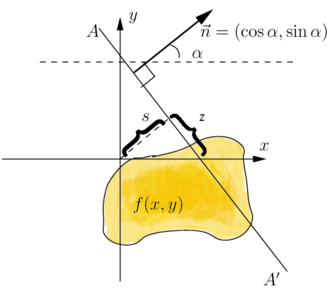
\includegraphics[scale=0.4]{images/radon} \texttt{\char32}
	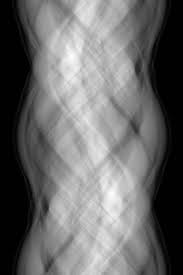
\includegraphics[scale=0.4]{images/sinogram} 
\end{frame}

\begin{frame}\frametitle{Projection-Slice Theorem }
	Зв'язок між перетворенням Фур'є та перетворенням Радона \linebreak
	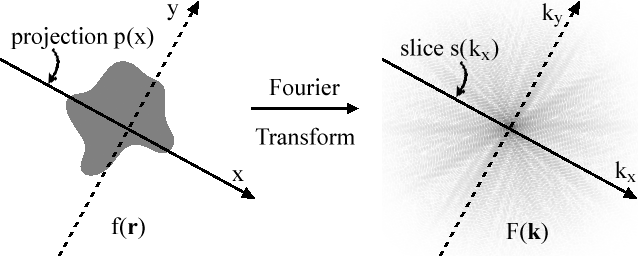
\includegraphics[scale=0.4]{images/projection_slice} 
\end{frame}

\begin{frame}\frametitle{Ridglet Transform }
	Це вейвлет-перетворення, застосоване до ліній у просторі Радона
	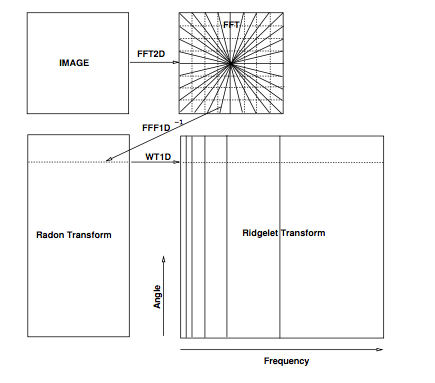
\includegraphics[scale=0.35]{images/ridgelet}	 
\end{frame}

\begin{frame}\frametitle{Ridglet Transform }
	Застосовано вейвлет Добеші D4 = [0.482962, 0.836516, 0.224143, -0.129409], висока та низька частота обчислюються за формулами: \linebreak
	high[v] = y[2*v]*D4[0] + y[2*v+1]*D4[1] + y[2*v+2]*D4[2] + y[2*v+3]*D4[3] \linebreak
	low[v] = y[2*v]*D4[3] - y[2*v+1]*D4[2] + y[2*v+2]*D4[1] – y[2*v+3]*D4[0]. \linebreak
	Вейвлет-коефіцієнти з абсолютним значенням меншим за заданий поріг σ встановлюються в 0, потім застосовується обернене перетворення.
\end{frame}

\begin{frame}\frametitle{Frequency Grid Tiling }
	Ridgelet-перетворення до областей у полярній системі координат \linebreak
	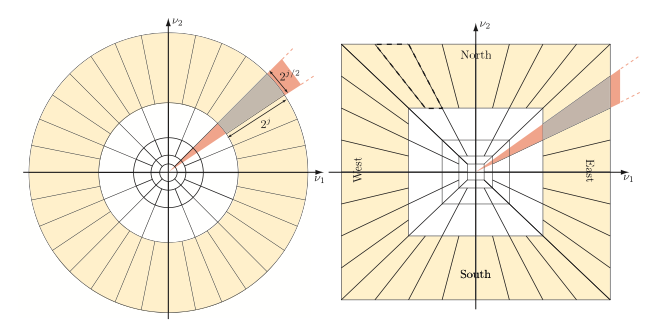
\includegraphics[scale=0.4]{images/grid_tiling} 
\end{frame}

\section{Використані технології}
\begin{frame}\frametitle{Використані технології: C++ та OpenGL}
	Переваги:
	\begin{enumerate}
		\item C++: швидкість обчислень  + гнучка архітектура
		\item GLSL: обчислення на GPU в десятки разів швидше  
	\end{enumerate}
	Недоліки:
	\begin{enumerate}
		\item GLSL: труднощі у відлагодженні програм
	\end{enumerate}

	Приклад коду шейдера:
	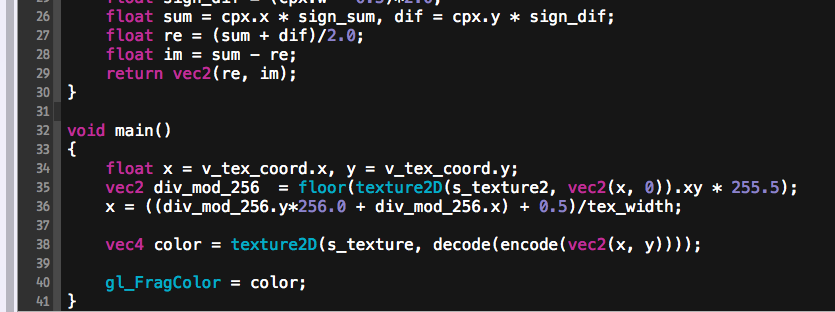
\includegraphics[height=2.5cm]{images/shader_snapshot}
\end{frame}

\begin{frame}\frametitle{Діаграма класів Curvelet Transform}
	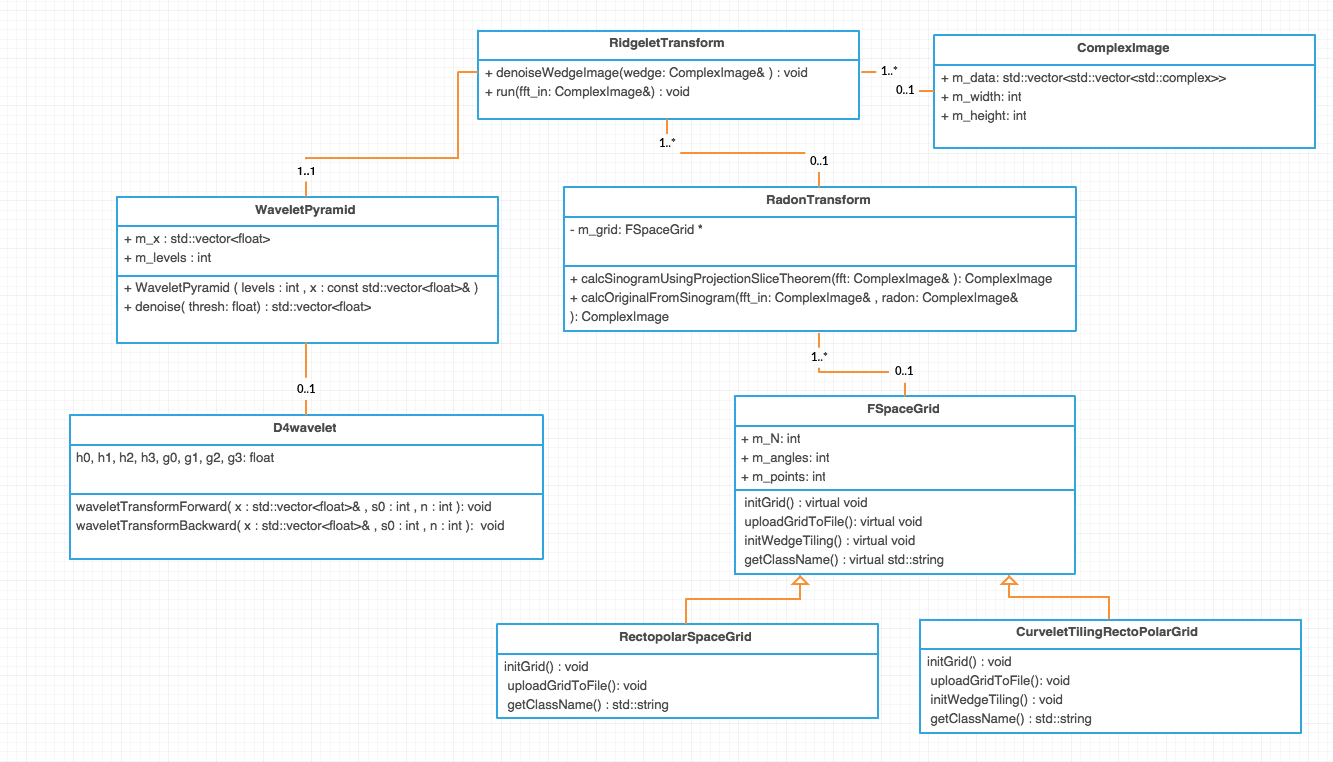
\includegraphics[scale=0.2]{images/class_diagram}
\end{frame}

\section{Поточні результати}
\begin{frame}\frametitle{Поточні результати}
	Зашумлене зображення(зліва) та результат роботи алгоритму(справа)
	\begin{center}
			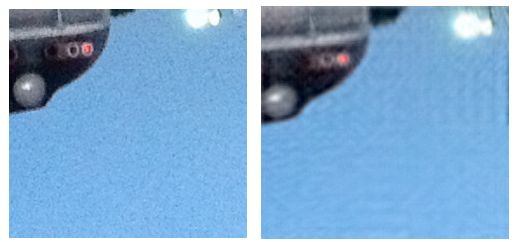
\includegraphics[width=8cm]{images/res_algo_1}
	\end{center}
\end{frame}
\begin{frame}\frametitle{Поточні результати}
	Зашумлене зображення(зліва) та результат роботи алгоритму(справа)
	\begin{center}
		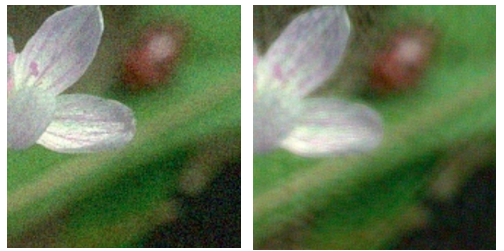
\includegraphics[width=8cm]{images/res_algo_2}
	\end{center}
\end{frame}

\section{Висновки}
\begin{frame}\frametitle{Висновки }
	\begin{enumerate}
		\item розроблено базову версію алгоритму Curvelet Transform
		\item буде покращено схему інтерполяції та обрано інший тип вейвлета
		\item це допоможе досягнути вищої візуальної якості 
	\end{enumerate}
\end{frame}

\begin{frame}\frametitle{}
	\begin{center}
	Дякую за увагу!
	\end{center}
\end{frame}


\end{document}
